\section[Magnetic impurities]{\texorpdfstring{Magnetic impurities in metals - \\ \null\hfill The Anderson and Kondo models}}


Imagine that we have a system defined by free, itinerant electrons, described by a conduction band with dispersion relation $\varepsilon_k$ and, for the sake of simplicity, assume that the one-particle density of state has a simple form as shown in Figure \ref{fig:dos}. The bandwidth of this system is $2D$, and the system has a Hamiltonian
\begin{equation}
	\label{eq:hamiltonian_free}
	\Ha_c = \sum_{k, \sigma}\varepsilon_k c_{k\sigma}^\dagger c_{k\sigma}.
\end{equation}

\begin{figure}[h]
	\centering
	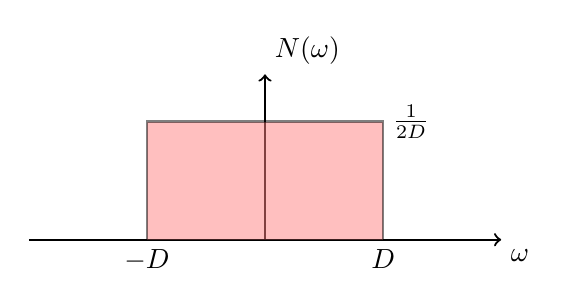
\begin{tikzpicture}[scale = 3]
	
	\draw[thick, ->] (0,1) -- (2,1);
	\draw[thick, ->] (1,1) -- (1,1.7);
	
	\draw[thick, draw = black,fill = red!50!white, opacity = 0.5] (0.5,1) rectangle (1.5,1.5);
	
	\node[anchor = north] at (0.5,1) {$-D$};
	\node[anchor = north] at (1.5,1) {$D$};
	\node[anchor = north west] at(2,1) {$\omega$};
	\node[anchor = south west] at (1,1.7){$N(\omega)$};
	\node[anchor = west] at (1.5, 1.5) {$\frac{1}{2D}$};
\end{tikzpicture}
	\caption{Density of states}
	\label{fig:dos}
\end{figure}

We will study the effect of including a magnetic impurity in the problem, where the magnetic impurity couples to the charged electrons, but is localized in space. First we consider the system with exactly one impurity. The Hamiltonian for this impurity is given by

\begin{equation}
	\Ha_f = E_0\sum_m f_m^\dagger f_m + U f_{\frac{1}{2}}^\dagger f_{-\frac{1}{2}}^\dagger f_{-\frac{1}{2}}f_{\frac{1}{2}},
\end{equation}

where $m$ are quantum numbers determining the z-component of the spin of the impurity. $(f_m, f_m^\dagger)$ are annihilation and creation operators for the impurity, in state $m$. $s = \frac{1}{2}: m = \pm 1$. $U$ is the Coulomb energy associated with double occupancy of the magnetic impurity. We will later assume that this is the largest energy in the system. The coupling between the charges and the localized impurity is given by
\begin{equation}
	\label{eq:interaction_term}
	\Ha_{cf}= \sum_{\vb k,\sigma,m}\left(V_{m\sigma}(\vb{k}) f_m^\dagger c_{\vb k\sigma}  + \text{h.c.}\right).
\end{equation}

In \eqref{eq:interaction_term}, $V_{m\sigma}(\vb k) $ is the matrix element transfering an electron from the impurity to the conduction band, or opposite. 
The total Hamiltonian is
\begin{equation}
	\Ha = \Ha_c + \Ha_f + \Ha_{cf}.
\end{equation}
$\Ha$ is often called the Anderson model. This model is the fundament for our understanding of heavy fermion systems. We will now use the techniques to study the effects of including a magnetic impurity in the conduction band. 
One important effect of magnetic impurities is that a metal will exhibit a minima in resistivity (see Figure \ref{fig:resistivity}).
\begin{figure}
	\centering
	\begin{tikzpicture}
    \begin{axis}[
        xmin = 0, xmax = 2,
        ymin = 0,% ymax = 1,
        axis lines = center,
        axis on top =true,
        domain = 0.1:1.6,
        %restrict y to domain=0:1,
        ylabel = $\rho(T)$,
        y label style={anchor=east},
        xlabel = $T$,
        xtick ={1},
        xticklabels={$T_K$},
        ytick style={draw=none},
        yticklabels={,,},
        samples = 100,
        %ticks = none
        ]
        
        \addplot[mark = none, draw = red!50!white, ultra thick]{1 -5*ln(x) + x^5};
        
        %\addplot[mark = none, draw = red!50!white, dashed]{1 -5*ln(x)};
        %\addplot[mark = none, draw = red!50!white, dashed]{x^5};
        
    	%\draw [thick] (axis cs:1.25,0)-- (axis cs:1.25,0.21);
    
        \node at (axis cs:0.6,5.5) {\footnotesize $\sim\ln T$};
        \node at (axis cs:1.25,6) {\footnotesize $T^5\sim $};
       	%\node[anchor = south] at (axis cs:1, 0) {$T_K = $ Kondo temperature};
        %\draw[->] (axis cs:3, 0.35) --(axis cs:4, 0.35) ;
    \end{axis}
\end{tikzpicture}
	\caption{Resistivity}
	\label{fig:resistivity}
\end{figure}
$T_K$ is only a couple of Kelvin, but the Fermi-energy is of order $10^4\mathrm{K}$. How can an energy scale this small arise when the basis is that the relevant energy scale is $\varepsilon_F \sim 10^4\mathrm{K}$? If magnetic impurities are excluded, the resistivity is uniformly decreasing. Jun Kondo found that $\rho(T) \sim -\ln T$ diverges in perturbation theory at low temperatures\footnote{Progress of Theoretical Physics, Vol. 32, No. 1, pp. 37-49}. A new problem then arises; how can we give a consistent description of low temperaturre physics, $T<<T_K$, in systems with a minima in resistivity? This problem is often referred to as the ``Kondo problem''. 

What we will do, is to see how the energy scale $T_K$, The Kondo temperature, arises, as well as to give a consistent description of the lowæ-temperature physics in metals doped with magnetic impurities, in a saddle point approxiimation.
Typical materials described by these theories are metals like aluminium and gold, doped with other rare materials. These materials are then the magnetic impurities in the problem. Rare materials: Lanthanides and actinides. Most studied: Cerium (Lanthanide) and Uranium (actinide). In the lanthanides the valence electrons are in the 4f-shell, and in actinides they are in the 5f-shell (hence $f_m^\dagger, f_m)$). Regularly studied materials are $\mathrm{CeAl_2}$ (lanthanide) and $\mathrm{UPt_3}$ (Actinide). $\mathrm{UPt_3}$ is a very odd superconductor with $T_C \sim 1\mathrm{mK}$ and a very complicated order parameter.  

